\subsection{Scrum of scrums}\label{sub:scrum-of-scrums}
Scrum of Scrums is a framework for scaling scrum across an organization. 
The ECDAR-SW5 organization uses Scrum of Scrums, as it allows each scrum team freedom to operate independently while providing a structure for communication \cite{spanner_scrum_nodate}. 

%In scrum of scrums we do not have daily scrums because the daily scrums is held in the smaller groups.
The daily scrum is a daily event, and because of that it would be impossible to get everyone together in the scrum of scrums every day for a daily scrum meeting.
Based on that we do not have daily scrums in the scrum of scrums.
%Working in scrum of scrums allows us as an organization to only hold daily scrum in each individual group, rather than across the entire organization.
%This simplifies the entire work process, ensuring focus. 
The key events in scrum of scrums are the sprint planning, sprint review, and sprint retrospective, and these events are handled by representatives of each group, which ensures that all groups have some insight into the overall process.
See \autoref{fig:scrum-of-scrums-events} for a more detailed look of the different events between scrum and scrum of scrums.

The multi-project is separated into two parts. 
There are five project groups working with the Reveaal engine, and one group working with GUI.
Each group has chosen a member to attend the scrum of scrums meetings as a representative of the group.
The reasoning for this was the number of members attending the meetings would get to big if every group member attended. 
The idea behind this was to keep the meetings as short as possible, and because of this, each group should hold a meeting internally after the sprint planning and before the review and retrospective. This ensures the representative is ready for the main scrum of scrums meeting. This process is also described in the figure below \ref{fig:scrum-of-scrums-events}.

%sending their committee to the main meeting for the scrum of scrums. 
%Based on that the groups choose a committee to attend the scrum meetings.

\begin{figure}[H]
    \centering
    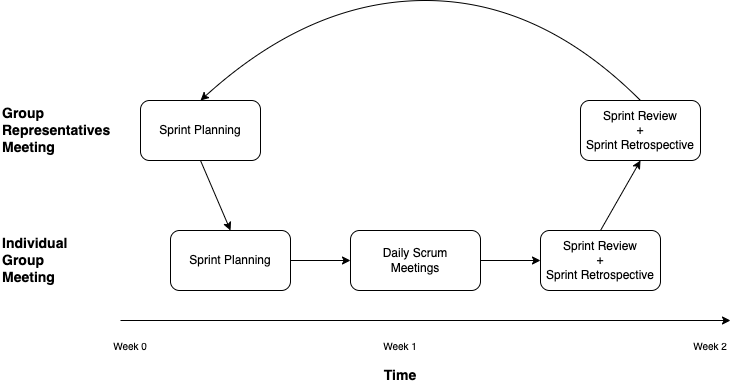
\includegraphics[width=\textwidth]{common/figures/Scrum_of_scrums_schedule.png}
    \caption{A figure depicting the events in a scrum sprint, divided between the big scrum of scrums group and the smaller scrum groups.}
    \label{fig:scrum-of-scrums-events}
\end{figure}


As mentioned, the multi-project focuses on both the GUI and Reveeal engine.
Because of this dual focus, we have two product owners: one product owner for the Reveaal teams and one for the GUI team.
The project's different product owners will help upholding the product backlog and update it if any changes appears. 
These changes are discussed during the scrum of scrums meetings, where the product owners can also be present.

The length of a sprint is measured against the length of the smaller scrum group's sprints.
Because of this, the average sprint length is two weeks.
Based on the length of the sprint, the scrum of scrums group has two meetings every two weeks. 
One meeting is for planning the upcoming sprint, and one is for sprint reviewing and retrospective at the end of a sprint.
These meetings, if possible, are held on the first Monday of a sprint, and the last Friday of a sprint, respectively.

% One for planing the upcoming sprint the first monday of the sprint, if possible and one meeting on last friday of the sprint, if possible.
% The last meeting's topics are always sprint reviewing and sprint retrospecting. 

